\documentclass[letterpaper,12pt]{article}

\usepackage{threeparttable}
\usepackage{geometry}
\geometry{letterpaper,tmargin=1in,bmargin=1in,lmargin=1.25in,rmargin=1.25in}
\usepackage[format=hang,font=normalsize]{caption}
\usepackage{amsmath}
\usepackage{mathrsfs}
\usepackage{multirow}
\usepackage{array}
\usepackage{delarray}
\usepackage{amssymb}
\usepackage{amsthm}
\usepackage{lscape}
\usepackage{natbib}
\usepackage{setspace}
\usepackage{float,color}
\usepackage[pdftex]{graphicx}
\usepackage{pdfsync}
\usepackage{verbatim}
\usepackage{placeins}
\usepackage{geometry}
\usepackage{pdflscape}
\synctex=1
\usepackage{hyperref}
\hypersetup{colorlinks,linkcolor=red,urlcolor=blue,citecolor=red}
\usepackage{bm}

\theoremstyle{definition}
\newtheorem{theorem}{Theorem}
\newtheorem{acknowledgement}[theorem]{Acknowledgement}
\newtheorem{algorithm}[theorem]{Algorithm}
\newtheorem{axiom}[theorem]{Axiom}
\newtheorem{case}[theorem]{Case}
\newtheorem{claim}[theorem]{Claim}
\newtheorem{conclusion}[theorem]{Conclusion}
\newtheorem{condition}[theorem]{Condition}
\newtheorem{conjecture}[theorem]{Conjecture}
\newtheorem{corollary}[theorem]{Corollary}
\newtheorem{criterion}[theorem]{Criterion}
\newtheorem{definition}{Definition} % Number definitions on their own
\newtheorem{derivation}{Derivation} % Number derivations on their own
\newtheorem{example}[theorem]{Example}
\newtheorem{exercise}[theorem]{Exercise}
\newtheorem{lemma}[theorem]{Lemma}
\newtheorem{notation}[theorem]{Notation}
\newtheorem{problem}[theorem]{Problem}
\newtheorem{proposition}{Proposition} % Number propositions on their own
\newtheorem{remark}[theorem]{Remark}
\newtheorem{solution}[theorem]{Solution}
\newtheorem{summary}[theorem]{Summary}
\bibliographystyle{aer}
\newcommand\ve{\varepsilon}
\renewcommand\theenumi{\roman{enumi}}
\newcommand\norm[1]{\left\lVert#1\right\rVert}
\usepackage{dcolumn}
\usepackage{booktabs}
\captionsetup{skip=0.333\baselineskip}
\newcolumntype{d}[1]{D{.}{.}{#1}}
\newcommand\mc[1]{\multicolumn{1}{@{}c@{}}{#1}}
\usepackage[format=plain,
            font=it]{caption}

\begin{document}

\title{A Sample JFE Paper\footnotetext{Financial support from \ldots}}

\author{Richard Stanton\\
  U.C. Berkeley}

\date{}              % No date for final submission

% Create title page with no page number

\renewcommand{\thefootnote}{\fnsymbol{footnote}}

\singlespacing

\maketitle

\vspace{-.2in}
\begin{abstract}
\noindent There's nothing very interesting here, but the format (achieved using the file \texttt{jfe.sty}) makes it suitable for publication in the \emph{Journal of Financial Economics} even if the content doesn't. Here's a nice, informative, single-spaced abstract.
\end{abstract}

\medskip

\noindent \textit{JEL classification}: XXX, YYY.

\medskip
\noindent \textit{Keywords}: \LaTeX; papers with no content.

\thispagestyle{empty}

\clearpage

\onehalfspacing
\setcounter{footnote}{0}
\renewcommand{\thefootnote}{\arabic{footnote}}
\setcounter{page}{1}

\section{Introduction}

The JFE likes the first section to have a title. The first line of each section is indented using the \texttt{indentfirst} package.\footnote{Here's a sample footnote.} Let's put in some sections and subsections to see how they get formatted.

\section{The Model} \label{sec:Model}

The baseline theoretical framework used here is similar to the one employed in Ackigit and Kerr (2016) and Acemoglu et al. (

\subsection{A Subsection}

In order to confirm the results from the maximum likelihood estimation, a second estimation routine was created using the Generalized Method of Moments. The adopted strategy was to estimate $\hat{\theta}_{GMM} = (\tau + \lambda_{int,abr}, \lambda_{inc,0}, \alpha)$ by solving equation~\eqref{eq:GMM} with the actual and the estimated moments ($m^d(x)$ and $m^e(x|\theta_{GMM})$, respectively, where $x$ is the real data).

\begin{equation} \label{eq:GMM}
\mathscr{L}(\theta_{GMM}) =  min_{\theta_{GMM}}e(x|\theta_{GMM})^TWe(x|\theta_{GMM})
\end{equation}

\noindent where $W$ is the weighting-matrix ($W = I$ here) and $e(x|\theta_{GMM})$ is the moment error function, defined as

\begin{equation} \label{eq:GMM_error}
e(x|\theta_{GMM}) \equiv \frac{m^e(x|\theta_{GMM}) - m^d(x)}{m^d(x)}
\end{equation}

In order to estimate those 3 parameters over the distribution of citations, a set of 4 moments was used: the average number of citations, the average of the first 5 sequential share ratios (e.g. \# of patents with 1 citation/\# of patents with 0 citations), the sum of the first two shares and the incremental R\&D intensity, defined in equation~\eqref{eq:RDintens} similarly to Akcigit and Kerr (2016).

\begin{equation} \label{eq:RDintens}
\texttt{R\&D intensity} = \frac{\beta\xi_{inc}\displaystyle\sum_{k=0}^{\infty}\eta_k\lambda_{inc,k}^2}{share_{inc}\pi}
\end{equation}

\noindent where $\beta = 0.106$ and $\pi = 0.0755$ are calibrated parameters from the general equilibrium and $\xi_{inc} = 0.346$ is the incremental R\&D scale (also calibrated).

Although no single parameter can be singled out with one particular moment, each of the proposed moments has an underlying intuition behind it:

\begin{itemize}
	\item The average number of citations and the R\&D intensity: two global measures of mass that, together, allow for the identification of $(\tau + \lambda_{int,abr})$ and $\lambda_{inc,0}$;
	\item Mean of the initial ratios: given that the initial incremental R\&D effort is a few times bigger than the creative destruction ($(\tau + \lambda_{int,abr})$), one would expect the initial reduction of incremental innovation to be related with the decay parameter $\alpha$;
	\item Sum of the first 2 bins: due to the presence of a significant discontinuity at zero citations (after all, "having ideas" is a highly skewed business), this moment adds an extra weight so as to pin down that effect.
\end{itemize}

The results of the estimation can be seen in Table \ref{GMMTable}. The overall estimation comes fairly close to matching all the data moments, while the estimated parameters are similar to the ones obtained with the MLE. As before, those results are robust to different initial conditions and to a "basin hopping" search. The estimation plot over the data histogram is available in the Appendix.

\begin{table}[htbp] \centering \captionsetup{width=5.8in}
    \caption{\label{GMMTable}\textit{Estimated and data moments using the Generalized Method of Moments}}
	\centering
	\begin{tabular}{l llp{1.5cm} p{0.5cm} llp{1.5cm}}
	\toprule
	Moment & \multicolumn{1}{c}{Data} & \multicolumn{1}{c}				{Model} \\ 
	\midrule
	Mean of citations & 10.06 & 7.39\\
	Mean of first 5 seq. ratios & 0.57 & 0.88\\
	Sum of first 2 bins & 0.26 & 0.22\\
	R\&D Intensity & 0.068 & 0.068\\
	Criterion & & 0.386\\
	\midrule
	$(\hat{\tau} + \hat{\lambda}_{int,abr}, \hat{\lambda}_{inc,0}, \hat{\alpha}) = (0.047, 0.351, 1)$\\
	\bottomrule
	\end{tabular}
\end{table}

To test for robustness on both GMM and MLE, we have also checked the predictions of both models on an untargeted moment: the share of incremental R\&D effort over total effort. Results can be seen in table \ref{Untarg}. Both models presented a close match to the value observed in the data.

\begin{table}[htbp] \centering \captionsetup{width=5.8in}
    \caption{\label{Untarg}\textit{Estimated and actual results for the untargeted share of incremental R\&D effort}}
	\centering
	\begin{tabular}{l llp{1.5cm} p{0.5cm} llp{1.5cm}}
		\toprule
		Moment & \multicolumn{1}{c}{Data} & \multicolumn{1}{c}				{Model} \\ 
		\midrule
		MLE\\
		\;Incremental/total & 0.90 & 0.91\\
		GMM\\
		\;Incremental/total & 0.90 & 0.88\\
		\bottomrule
	\end{tabular}
\end{table}

Nothing very odd about the formatting of section and subsection headings. Here's a reference to Section~\ref{sec:subsec} or~\ref{sec:subsub}. Let's also add some parenthetical citations (see~\citealp{Stanton:95,CarpenterStantonWallace:12}; and \citealp{Campbell:03}). 

To justify adding a subsection here, from now on, we'll assume
\begin{condition}\label{cond:rates}
$0 <  \hat{\mu} < \gamma\sigma^2$.
\vspace{3mm}
\end{condition}
This condition might be useful if there was a model. 

\subsection{Another Subsection, With a Figure}
\label{sec:subsec}

Figures get put at the end, with a note marking where they should go in the text, like this:

\bigskip
\centerline{\bf [Insert Figure~\ref{fig:0} near here]}
\bigskip

\subsubsection{A Subsubsection with a Proposition}
\label{sec:subsub}

Let's put a proposition here.
\begin{proposition} \label{prop:3}
If Condition~\ref{cond:rates} is satisfied,  a solution to the central
planner's problem, $V(B,D,t) \in C^2\left( {\mathbb R}_{+}^2 \times
  [0,T] \right)$, with control $a:[0,1]\times[0,T]\rightarrow [-\lambda,\lambda]$
 if  $\gamma>1$ is
\begin{equation} \label{eq:valuea}
V(B,D,t) =  - \frac{(B+D)^{1-\gamma}}{1-\gamma}   w\left(\frac{B}{B+D},t\right).
\end{equation}
\end{proposition}

% Bibliography.

\bibliographystyle{jfe}
\bibliography{Paper}

\clearpage

\appendix

\section{An Appendix}
\label{sec:app1}

Here's an appendix with an equation. Note that equation numbering continues where it left off in the main body and that the JFE wants the word ``Appendix'' to appear before the letter in the appendix title. This is all handled in \texttt{jfe.sty}.

\begin{figure}[htb]\centering \captionsetup{width=5.8in}
    \fbox{\resizebox{4.0in}{2.7in}{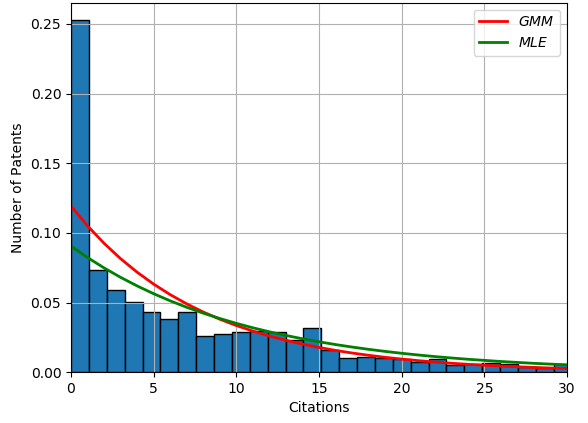
\includegraphics{GMM_MLE.png}}}
    \caption{\label{GMM_MLE}\textit{Citation distribution for same-class abrupt patents and estimation results for MLE and GMM}}
\end{figure}

\end{document}
